\mysection[black]{6. Flow \& GC}


\mysubsection{6.1 Control Flow}
\textbf{Block}: Single entry point, seq. of (possibly empty) instr, ends with single control-flow instr.\\
\textbf{Control-Flow Graph (CFG)}: Nodes are blocks, $E(b_1,b_2)$ iff $b_1$ may jump to $b_2$\\
\textbf{Domination}: $A$ dominates $B$: if the only way to reach $B$ from start node is via $A$\\
\textbf{Back Edge}: Edge in CFG where target dom the source $E(n,h) \wedge n \in \operatorname{dom}[h]$, $h$=header, \textcolor{red}{be aware: transitive !} \\
\textbf{Natural Loop (NL)}: Given back edge $E(n,h)$, NL is set of nodes dominated by $h$, that can reach (in CFG) $n$ without passing through $h$ $\cap \{h\}$ \\
\textbf{Dominator Dataflow Analysis (DDA)}: Computed using a forward, must dataflow anal.\\
\textbf{Algorithm for DOM-Trees}: 
\begin{enumerate}[leftmargin = *,noitemsep]
\item  Init $\operatorname{dom}[\operatorname{entry}]=\{\operatorname{entry}\}$,$\operatorname{dom}[n]=\{\forall n \in \operatorname{CFG}\}$
\item Iter. until conv. $\operatorname{dom}[n] = \{n\}\cup \bigcap_{p\in \operatorname{pred}[n]}\operatorname{dom}[p]$
 \end{enumerate}
\textbf{Dom-Trees (DT)}: All CFG have DT, built through DDA, properties: transitive $A  \operatorname{dom} B \vee B  \operatorname{dom} C\Rightarrow A  \operatorname{dom} C$, anti-symmetric $A  \operatorname{dom} B \vee B  \operatorname{dom} A\Rightarrow A = B$\\
\textbf{Dominance Frontier (DF)}: of a node $B$ is the set of all CFG nodes $y$ such
that $B$ dominates a predecessor of $y$, but does not strictly dominate $y$\\
\textbf{Algo (from CFG)}: $\forall n: \forall p \in \operatorname{pred}[n] \left(\right.r = p;$ $ \operatorname{while}(r \neq \operatorname{doms}[B])\left\{ \operatorname{DF}[r]:= \operatorname{DF}[r] \cup B; r:= \operatorname{DF}[r]\right\}\left.\right)$\\
\textbf{Algo (from DF)}: Given nodes $N$, compute $\operatorname{DF}[S]=\bigcup_{n \in N} \operatorname{DF}[n]$ Repeat until convergence: $S \leftarrow S \cup \operatorname{DF}(S)$\\

\mysubsection{6.2 Data Flow (DF)}
\textbf{DF Anal.}: Compute liveness $\forall$ vars. simult.\\
\textbf{Use/Def}: $\operatorname{use}[s]$/$\operatorname{def}[s]$ set of var. used/defined by $s$\\
\textbf{In/Out}: $\operatorname{in}[n]$/$\operatorname{out}[n]$ set of var. live on entry/exit of $n$\\
\textbf{Gen/Kill}: $\operatorname{gen}[n]$/$\operatorname{kill}[n]$: info. generated/invalidated by $n$ \\


\textbf{Liveness}: Variable $v$ is live on edge $e$ if:
\begin{enumerate} [leftmargin = *,noitemsep]
\item a node $n$ in the CFG such that $v\in \operatorname{use}[n]$, and
\item a dir. path $P(e,n)$ s.t $\forall s' \in P(e,n)\Rightarrow v \not \in \operatorname{def}[s']$
\end{enumerate}
\textbf{Computational Inference Conditions}:

\begin{multicols}{2}
\begin{center}
    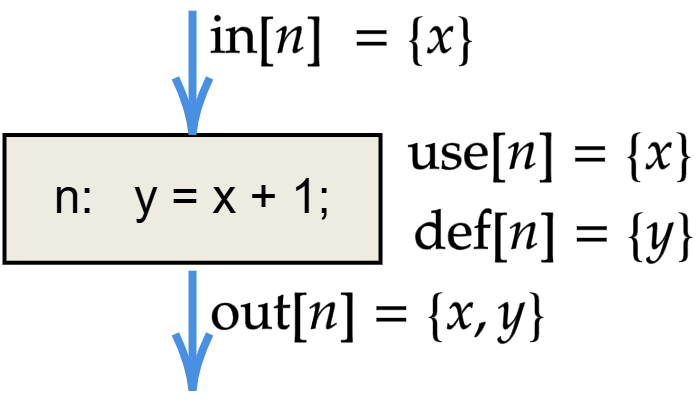
\includegraphics[width=0.75\linewidth]{images/defs.png}
\end{center}
\columnbreak
\begin{enumerate} [leftmargin = *,noitemsep]
\item $\operatorname{in}[n] \supseteq \operatorname{use}[n]$
\item $\operatorname{in}[n] \supseteq \operatorname{out}[n]\operatorname{def}[n]$
\item $\operatorname{out}[n] \supseteq  \operatorname{in}[n'] \text{ if } n' \in\operatorname{succ}[n]$
\end{enumerate}
\end{multicols}

\textbf{Iter. Anal}: Start with $\operatorname{in}[n]=\operatorname{out}[n]=\emptyset$ and converge\\
\textbf{Algo}: Set $\forall n.\operatorname{in}[n]=\operatorname{out}[n]=\emptyset$. Repeat until guaranteed convergence i.e. no change in $\operatorname{in}$ and $\operatorname{out}$: {\footnotesize $\forall n. \left[ \operatorname{out}[n]=\bigcup_{n'\in \operatorname{succ}[m]}\operatorname{in}[n']\text{ then} \operatorname{in}[n]= \operatorname{use}[n] \cup \left(\operatorname{out}[n] \setminus \operatorname{def}[n]\right) \right]$ }\\

\textbf{Meet-Over-Path (MOP)}: Solution that accounts for all possible paths in the CFG: $\bigcap_{p \in \operatorname{paths_to}[n]}\ell_p$, where $\ell_p$ is dataflow info (liveness ...)\\
\textbf{Iter. Sol.}: Converges to MOP sol, if distributive $\bigcap_i F_n (\ell_i)= F_n (\bigcap_i \ell_i)$\\
\textbf{Distributive properties}: Program structure: liveness, available expr, reaching def, busy expr\\
\textbf{Non-Distr. prop.}: What is computed: output = pos. ?, constprop\\



\begin{center}
\begin{tabular}{lll}
\hline
\textbf{Analysis} & \textbf{Type} & \textbf{Equations} \\
\hline

Liveness &
BW, May &
{\tiny $
\begin{array}{l}
\text{out}[n] := \bigcup_{n' \in \mathrm{succ}[n]} \text{in}[n'] \\
\text{in}[n] := \text{use}[n] \cup (\text{out}[n] \setminus \text{def}[n])
\end{array}$}
\\[1.5ex]

Reaching Def. &
FW, May &
{\tiny $
\begin{array}{l}
\text{in}[n] := \bigcup_{p \in \mathrm{pred}[n]} \text{out}[p] \\

\end{array}$}
\\[1.5ex]

Available Expr. &
FW, Must &
{\tiny $
\begin{array}{l}
\text{in}[n] := \bigcap_{p \in \mathrm{pred}[n]} \text{out}[p] \\
\text{out}[n] := \text{gen}[n] \cup (\text{in}[n] \setminus \text{kill}[n])
\end{array}$}
\\[1.5ex]

Constant Prop. &
FW, May &
{\tiny $
\begin{array}{l}
\text{in}[n] := \bigcup_{p \in \mathrm{pred}[n]} \text{out}[p] \\
\text{out}[n] := \text{transfer}_n(\text{in}[n])
\end{array}$}
\\[1.5ex]

Alias Anal. &
FW, May &
{\tiny $
\begin{array}{l}
\text{in}[n] := \bigcup_{p \in \mathrm{pred}[n]} \text{out}[p] \\
\text{out}[n] := \text{transfer}_n(\text{in}[n])
\end{array}$}
\\

Busy Expr. &
BW, Must&
{\tiny $
\begin{array}{l}
\text{out}[n] := \bigcap_{p \in \mathrm{succ}[n]} \text{in}[p] \\
\text{in}[n] := \operatorname{gen}[n] \cup \left(\operatorname{out}[n] \setminus \operatorname{kill}[n]\right)
\end{array}$}
\\
\hline
\end{tabular}
\end{center}






\mysubsection{6.3 GC}
\textbf{Reachability}: $X$ is reachable iff A register contains a pointer to $X$, or another reachable object contains a pointer to $X$, approximation if object is used or not\\
\textbf{GC Scheme}: 1. Allocate space for new ojects, 2. Compute objects that might be used again, free space not in the found objects from before\\

\textbf{Mark and Sweep}: Each Object has mark bit ($1\Leftrightarrow$ reachable); When memory runs out, GC does: 1. Mark Phase: Trace reachable objects 2. Sweep Phase: Collect garbage object, add to free list, fragmentation possible\\
\textbf{Pointer Reversal}: Stackless graph traversal, temporarily reversing heap ptr, s.t. store the parent, when traversing back original pointer is restored\\
\textbf{Stop and Copy}: Mem. org. in 2 areas: Old- (OS) \& new Space (NS), Heap pointer points to next free word in OS. When OS is full: 1. Copy reachable objects into NS 2. Reverse role of NS and OS. , Generally fastest method, cannot be done in C, as copying is impossible\\
\begin{center}
    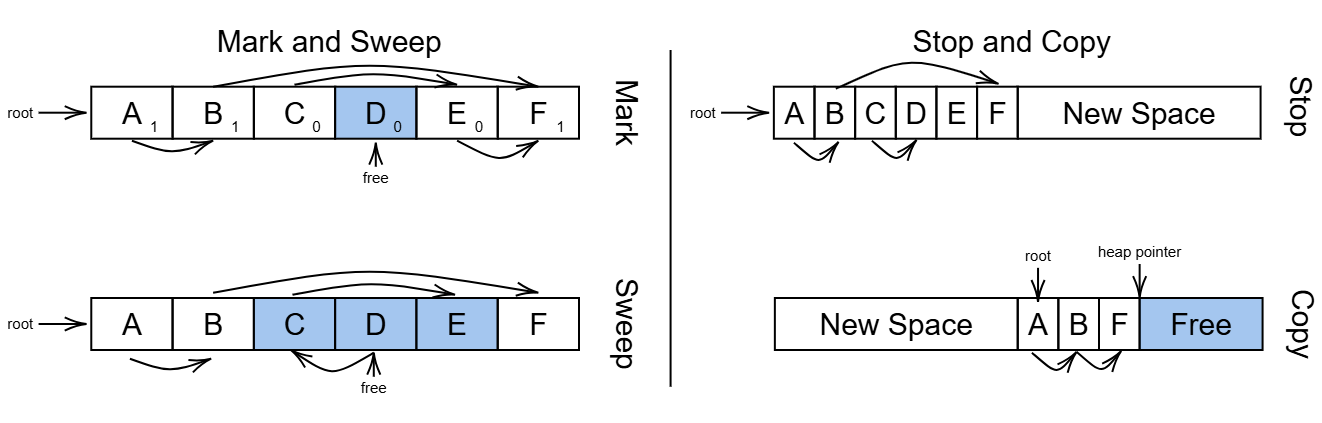
\includegraphics[width=1\linewidth]{images/gc.png}
\end{center}
\textbf{Reference Counting}: Keeps track of number of ptr to object, very slow, not possible for circular structures \\


